\chapter{Felhasználói dokumentáció} % User guide
\label{ch:user}

\section{Bejelentkezés és nyelvválasztás}
Az oldalra érkezve a kezdőoldalt láthatjuk, ahol egy üdvözlő üzenet fogad minket. Majd lehetőségünk nyílik bejelentkezni a rendszerbe, vagy a rendszer által támogatott lokalizációt tudjuk kiválasztani (\ref{fig:main-page} ábra). \footnote{Erre majd még a bejelentkezés után is lehetőségünk nyílik lásd később,~\hyperref[step:mindenkinek-elerheto-oldal]{\ref{step:mindenkinek-elerheto-oldal}:~``Mindenki számára elérhető oldalak''}}
\begin{figure}[H]
	\centering
	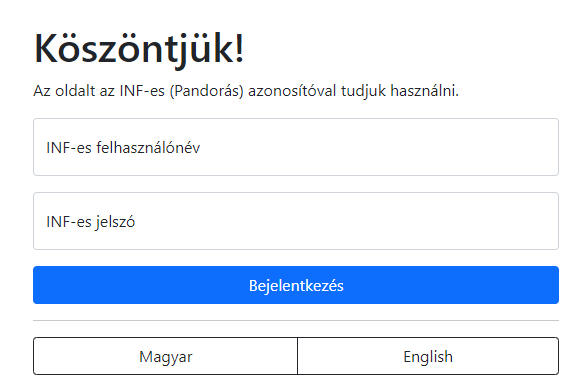
\includegraphics[width=0.6\textwidth]{userguide/main-page}
	\caption{Főoldal}
	\label{fig:main-page}
\end{figure}
\subsection{Bejelentkezés}
A rendszerbe bejelentkezni az INF-es felhasználónkkal tudunk. Ha a bejelentkezés sikertelen volt, azt a rendszer hibaüzenetekkel jelzi a számunkra (\ref{fig:login-error} ábra). 
\begin{figure}[H]
	\centering
	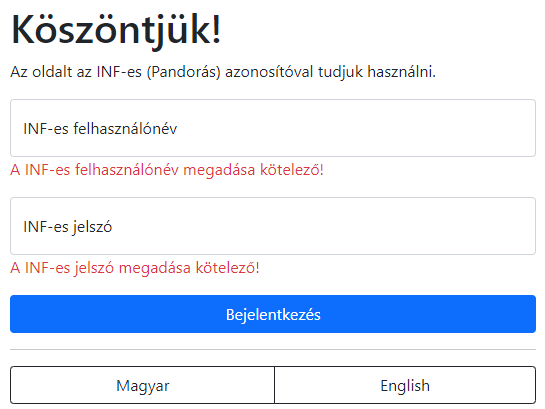
\includegraphics[width=0.6\textwidth]{userguide/login-error}
	\caption{Bejelentkezési hiba}
	\label{fig:login-error}
\end{figure}
Amennyiben a bejelentkezés sikeres volt, a \emph{szerepkörnek} megfelelő kezdőoldalon találjuk magunkat (\ref{fig:logged-in} ábra).
\begin{figure}[H]
	\centering
	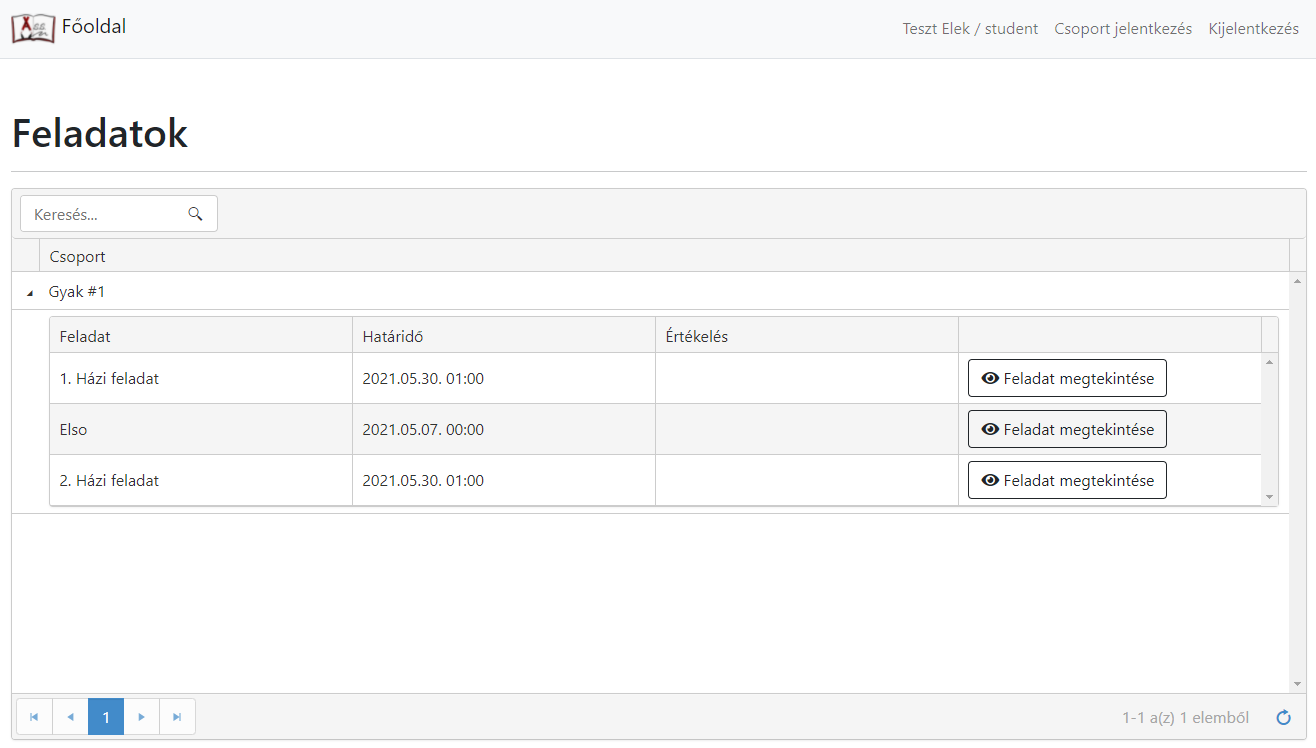
\includegraphics[width=1.0\textwidth]{userguide/logged-in}
	\caption{Sikeres bejelentkezés}
	\label{fig:logged-in}
\end{figure}
\subsection{Nyelvválasztás}
A rendszer kilistázza a támogatott lokalizációkat (jelenleg magyar és angol). Alapértelmezett beállítás a magyar. Ezt felültudjuk írni, ha valamelyik gombra rákattintunk. (\ref{fig:change-lang} ábra)
\begin{figure}[H]
	\centering
	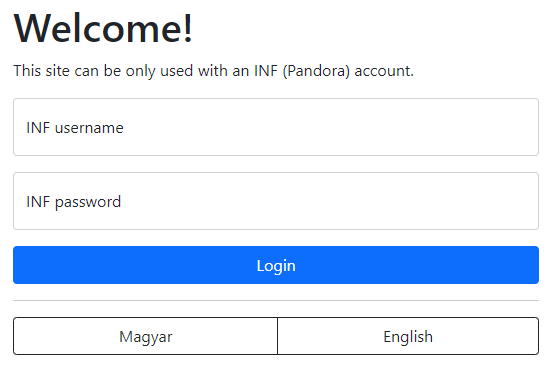
\includegraphics[width=0.6\textwidth]{userguide/change-lang}
	\caption{Nyelvváltás}
	\label{fig:change-lang}
\end{figure}
\section{Szerepkörök}
A felhasználók négy csoportba tartozhatnak:
\begin{compactitem}
    \item \hyperref[step:admin-role]{Rendszergazda}
    \item \hyperref[step:teacher-role]{Tárgyfelelős}
    \item \hyperref[step:instructor-role]{Gyakorlatvezető}
    \item \hyperref[step:student-role]{Hallgató}
\end{compactitem}
Egy felhasználó tartozhat több szerepkörbe. Ha egy felhasználó több szerepkörbe is tartozik, akkor a felület menüsorán megjelenik egy "Szerepkör váltás" lenyitható menü, ahol a felhasználóhoz rendelt szerepköröket találjuk, a kiválasztott linkre kattintva a csoporthoz tartozó kezdőoldalra navigáljuk magunkat. A felhasználóhoz a szerepköröket a felhasználó létrehozásakor is megadhatjuk, valamint a létrehozást követően tudjuk módosítani.
\subsection{Rendszergazda}\label{step:admin-role}
A rendszergazda a következő funkciókat érheti el:
\begin{compactitem}
    \item Tantárgy létrehozása, módosítása, törlése, tárgyi információk megtekintése
    \item Felhasználó létrehozása, módosítása, a felhasználók adatainak a megtekintése
\end{compactitem}
Ha rendszergazdaként jelentkezünk be az alábbi két táblázat fogad minket a kezdőoldalon~(\ref{fig:admin-page} ábra). 
\begin{figure}[H]
	\centering
	\subfigure[Tantárgyak táblázata]{
		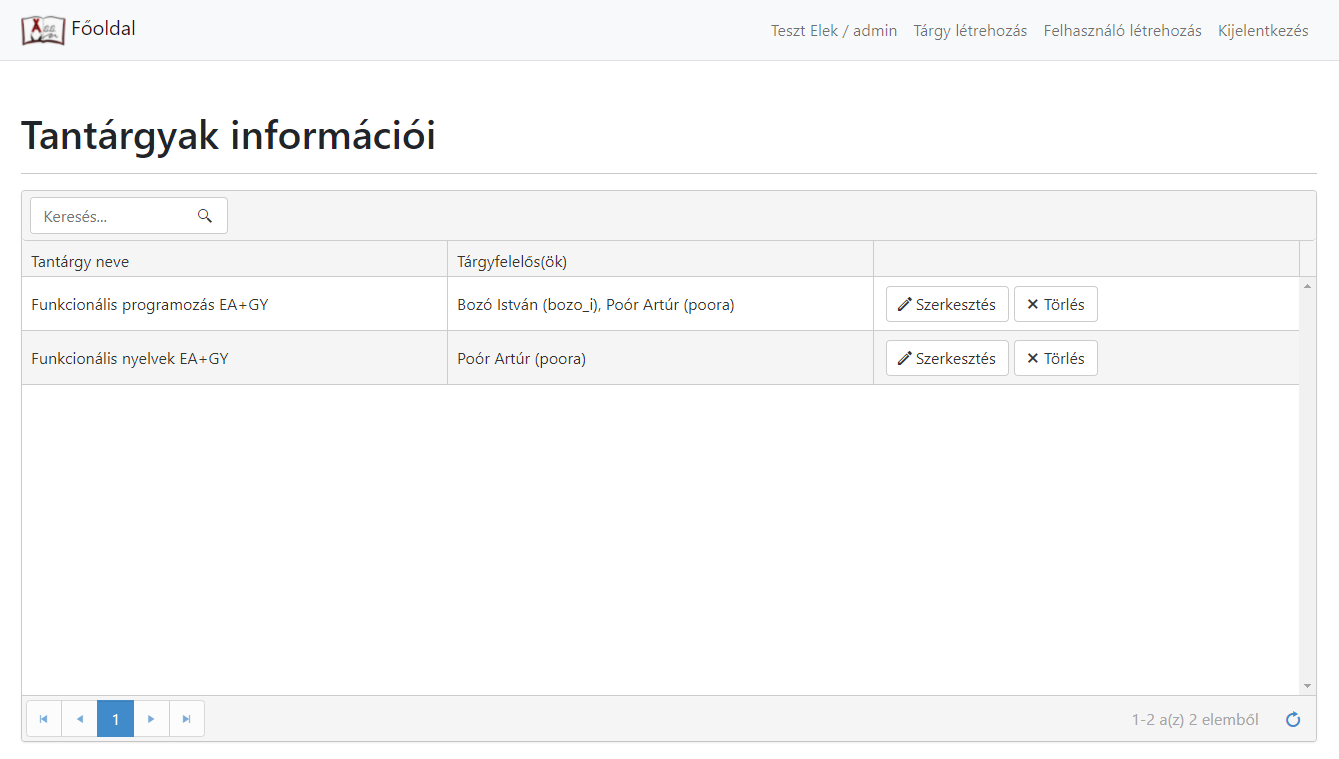
\includegraphics[width=1\linewidth]{userguide/admin-table1}
        \label{subfig:admin-subject-table}}
	\hspace{5pt}
	\subfigure[Felhasználók táblázata]{
		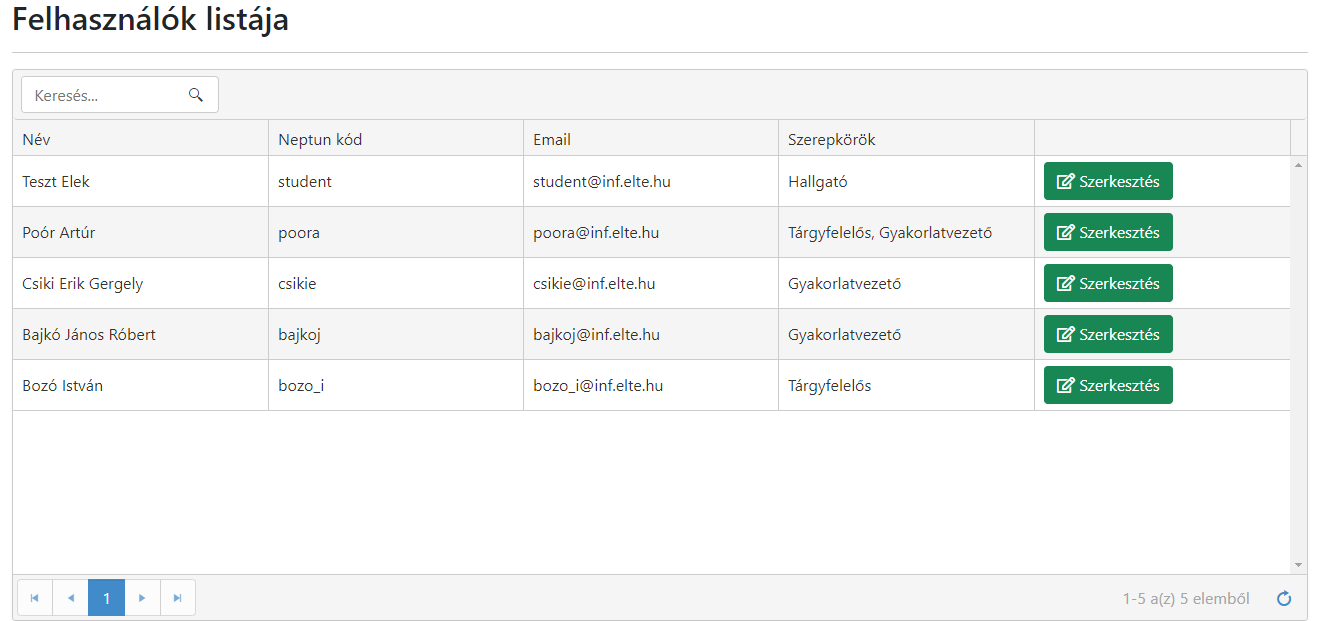
\includegraphics[width=1\linewidth]{userguide/admin-table2}
        \label{subfig:admin-users-table}}
	\caption{Rendszergazdai szerepkör kezdőoldala}
	\label{fig:admin-page}
\end{figure}
Az első táblázatban a rendszerben létrehozott tantárgyak és a hozzájuk tartozó információk olvashatóak le. A táblázatban az egyes tantárgyakhoz tartozó adatok módosíthatóak, illetve az egész tárgyat lehet törölni. A módosítás során validálásra kerül, hogy a módosított név létezik-e már a rendszerben, ha igen, akkor ezt a rendszer jelzi számunkra. A második táblázatban a rendszerben létrehozott felhasználókat és a hozzájuk tartozó információkat láthatjuk. A rendszergazda a felhasználók adatait és szerepköreit tudja módosítani.
\subsubsection{Tantárgy létrehozása}
A ``Tárgy létrehozás'' linkre kattintva az alkalmazás átnavigál minket egy űrlapra, ahol az új tantárgy szükséges adatait tudjuk kitölteni (\ref{subfig:admin-create-subject} ábra). Ha az adatok validálása és feldolgozása sikeres, akkor visszanavigálódunk a kezdőoldalra. Az esetleges validalási hibákat a rendszer jelzi számukra (\ref{subfig:admin-create-subject-error} ábra).
\begin{figure}[H]
	\centering
	\subfigure[Űrlap]{
		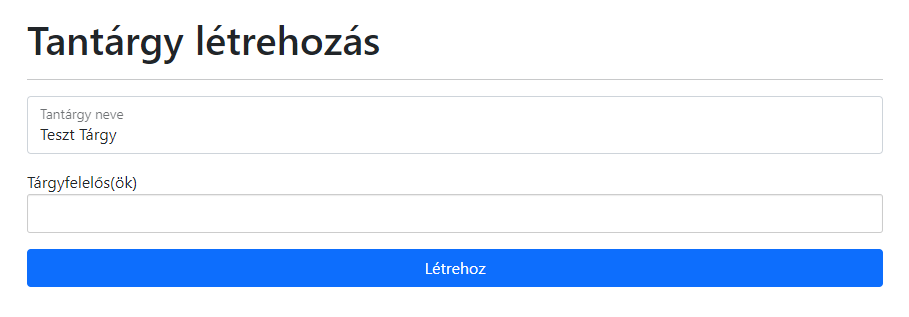
\includegraphics[width=0.8\linewidth]{userguide/admin-create-subject-form}
        \label{subfig:admin-create-subject}}
	\hspace{5pt}
	\subfigure[Adatok validálása]{
		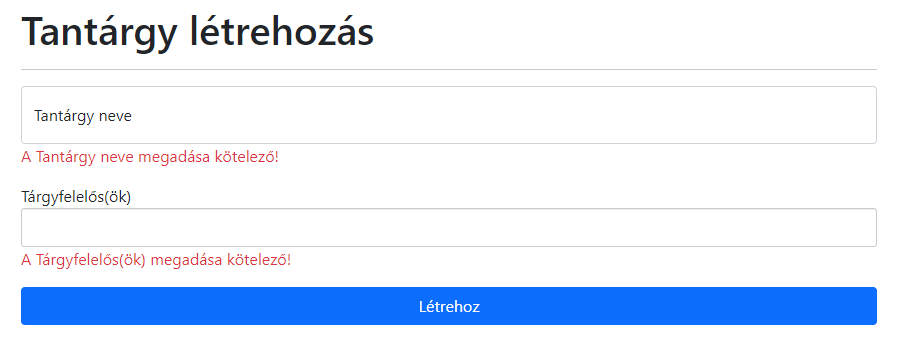
\includegraphics[width=0.8\linewidth]{userguide/admin-create-subject-error}
        \label{subfig:admin-create-subject-error}}
	\caption{Tantárgy létrehozás}
	\label{fig:admin-create-subject}
\end{figure}
\subsubsection{Felhasználó létrehozása}
Felhasználót létrehozni a ``Felhasználó létrehozás'' linkre kattintva tudjuk megtenni, ami továbbnavigál minket egy űrlapra, ahol az új felhasználónak az adatait tudjuk megadni (\ref{subfig:admin-create-user} ábra). Ha az adatok validálása sikeres, akkor a felhasználó elkészült és visszanavigálódunk a kezdőoldalra, ha nem volt sikeres, akkor a rendszer ezt hibaüzenetekkel jelzi nekünk (\ref{subfig:admin-create-user-error} ábra).
\begin{figure}[H]
	\centering
	\subfigure[Űrlap]{
		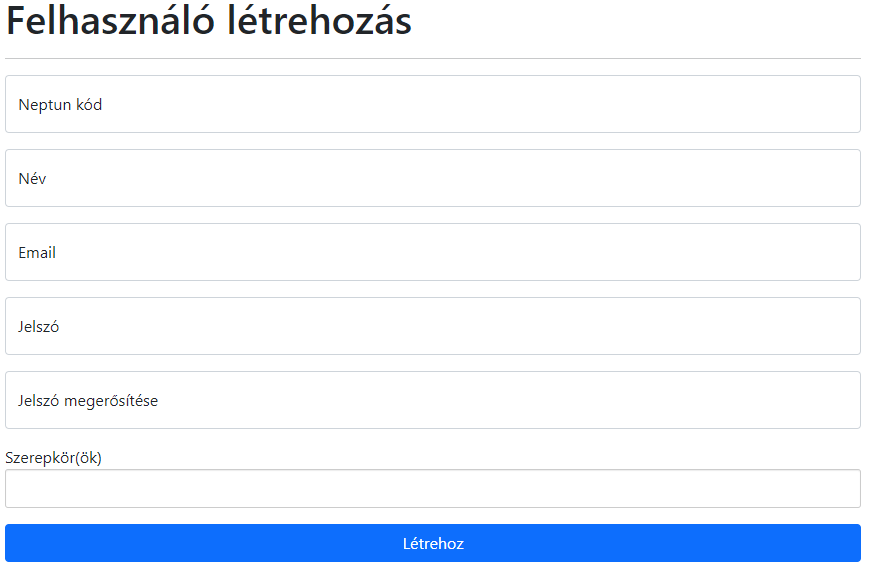
\includegraphics[width=0.7\linewidth]{userguide/admin-create-user-form}
        \label{subfig:admin-create-user}}
	\hspace{5pt}
	\subfigure[Adatok validálása]{
		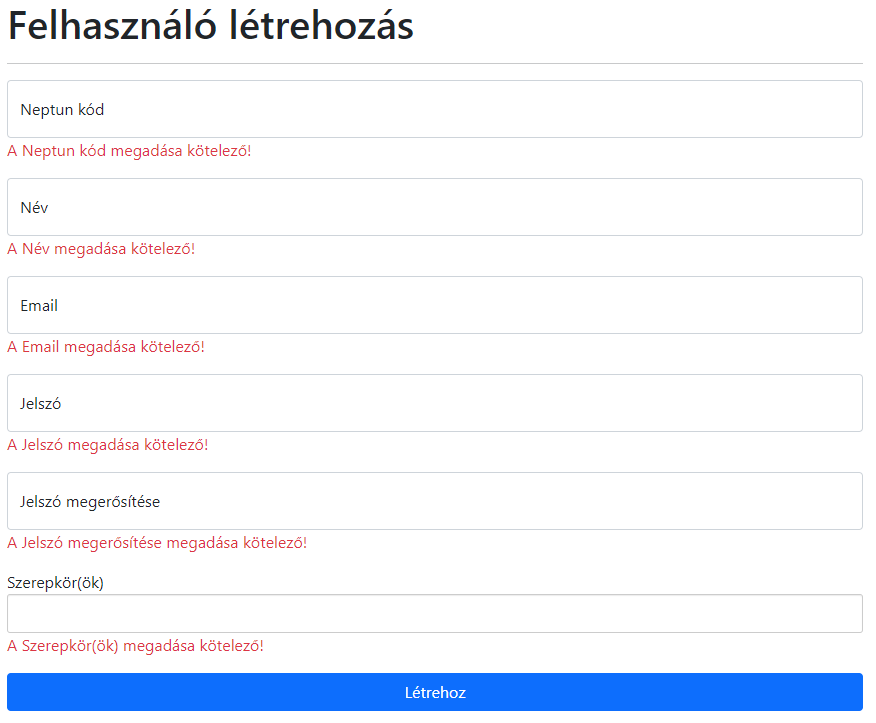
\includegraphics[width=0.85\linewidth]{userguide/admin-create-user-error}
        \label{subfig:admin-create-user-error}}
	\caption{Felhasználó létrehozás}
	\label{fig:admin-create-user}
\end{figure}
\subsection{Tárgyfelelős}\label{step:teacher-role}
Ha tárgyfelelősként jelentkezünk be a rendszerbe, akkor az alábbi kezdőoldal fogad minket (\ref{fig:teacher-home} ábra).
A kezdőoldalon egy tablázat található, amiben látjuk azokat a tantárgyakat, és a tantárgyakhoz tartozó csoportokat, amelyeknek a felelősei vagyunk.
A tárgyfelelős a következő funkciókat használhatja:
\begin{compactitem}
    \item \hyperref[step:teacher-create-course]{Csoport létrehozása egy tantárgyhoz}
    \item \hyperref[step:teacher-edit-course]{Csoport módosítása}
\end{compactitem}
\begin{figure}[H]
	\centering
	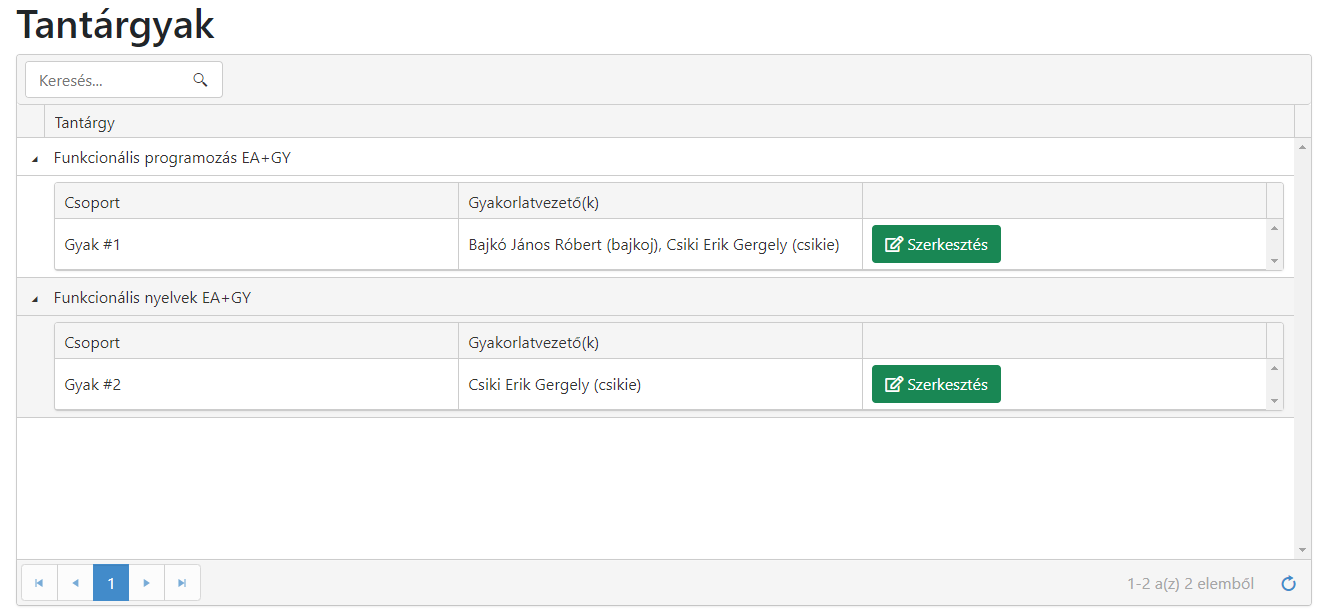
\includegraphics[width=1.0\textwidth]{userguide/teacher-home}
	\caption{Tárgyfelelős kezdőoldala}
	\label{fig:teacher-home}
\end{figure}
\subsubsection{Csoport létrehozása}
\label{step:teacher-create-course}
A menüsoron a ``Csoport létrehozás'' linkre kattintva a rendszer átirányít minket egy űrlapra, ahol létre tudunk hozni egy csoportot (\ref{fig:teacher-create-course} ábra). Az adatokat a rendszer validálja, és az esetleges hibákat jelzi számunkra.
\begin{figure}[H]
	\centering
	\subfigure[Űrlap]{
		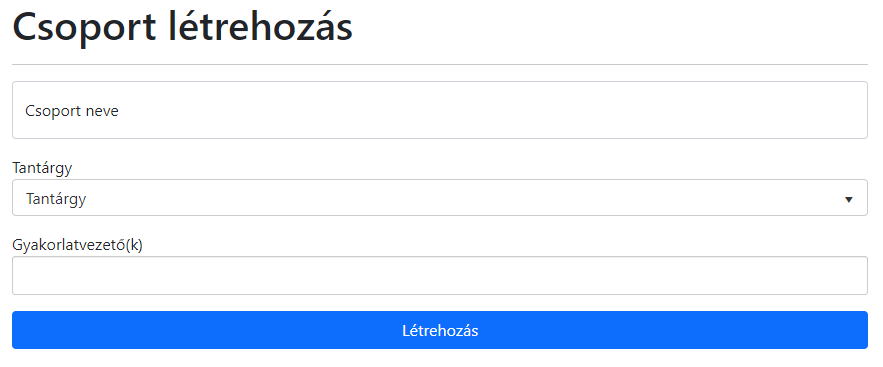
\includegraphics[width=0.75\linewidth]{userguide/teacher-create-course-form}
        \label{subfig:teacher-create-course-form}}
	\hspace{5pt}
	\subfigure[Adatok validálása]{
		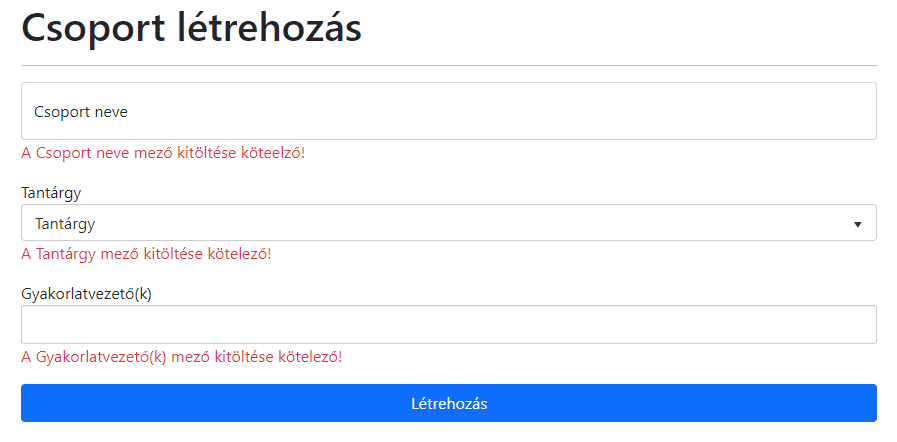
\includegraphics[width=0.75\linewidth]{userguide/teacher-create-course-error}
        \label{subfig:teacher-create-course-error}}
	\caption{Csoport létrehozás}
	\label{fig:teacher-create-course}
\end{figure}
\subsubsection{Csoport módosítása}
\label{step:teacher-edit-course}
Csoportokat szerkeszteni a kezdőoldalon található táblázat segítségével tudunk. A táblázatban lenyitható minden kilistázott tantárgy. Itt találjuk a tantárgyakhoz már létrehozott csoportokat. Minden tantárgy mellett találunk egy ``Szerkesztés'' gombot, melyre kattintva elérhetővé válik a csoport szerkesztése. Az adatok validálásra kerülnek, az esetleges hibákat a rendszer jelzi számunkra (\ref{fig:teacher-edit-course} ábra).
\begin{figure}[H]
	\centering
	\subfigure[Űrlap]{
		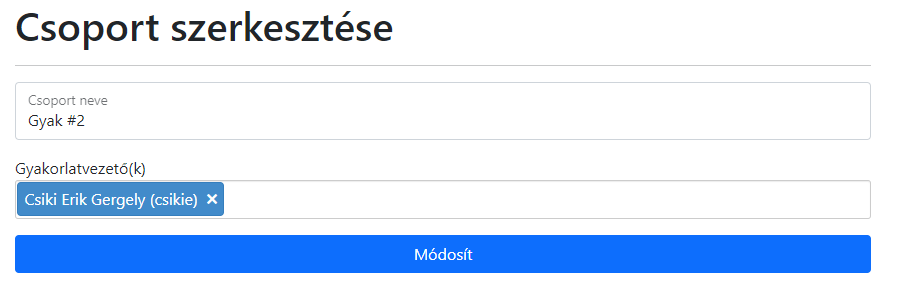
\includegraphics[width=0.75\linewidth]{userguide/teacher-edit-course-form}
        \label{subfig:teacher-edit-course-form}}
	\hspace{5pt}
	\subfigure[Adatok validálása]{
		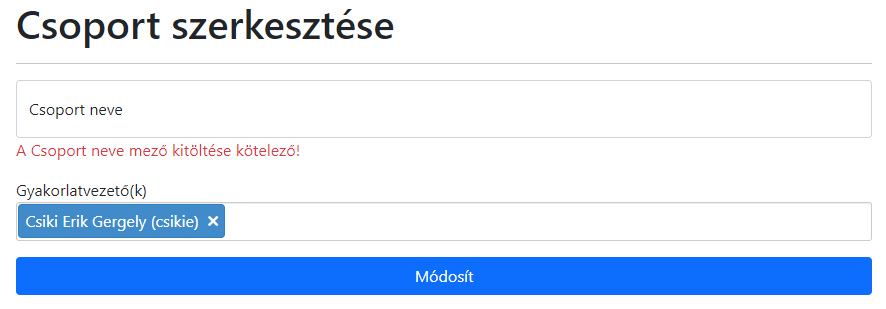
\includegraphics[width=0.75\linewidth]{userguide/teacher-edit-course-error}
        \label{subfig:teacher-edit-course-error}}
	\caption{Csoport módosítása}
	\label{fig:teacher-edit-course}
\end{figure}
\subsection{Gyakorlatvezető}\label{step:instructor-role}
Gyakorlatvezetőként bejelentkezve a rendszerbe a \ref{fig:instructor-home} ábrán látható kezdőoldal fogad minket. Az oldalon az ``Értékelendő beadandók'' cím alatt, a hozzánk rendelt csoportok hallgatóit láthatjuk egy-egy táblázatban, ahol láthatjuk, hogy egy hallgató az adott feladatra adott-e be megoldást. A ``Hallgatói várólista'' cím alatt szintén egy táblázatot találunk (\ref{subfig:instructor-table2} ábra), ahol tantárgyanként csoportosítva a következő információkat olvashatjuk le:
\begin{compactitem}
    \item Hallgató neve
	\item Hallgató neptun kódja
	\item Csoport neve
\end{compactitem}
\begin{figure}[H]
	\centering
	\subfigure[Értékelendő beadandók]{
		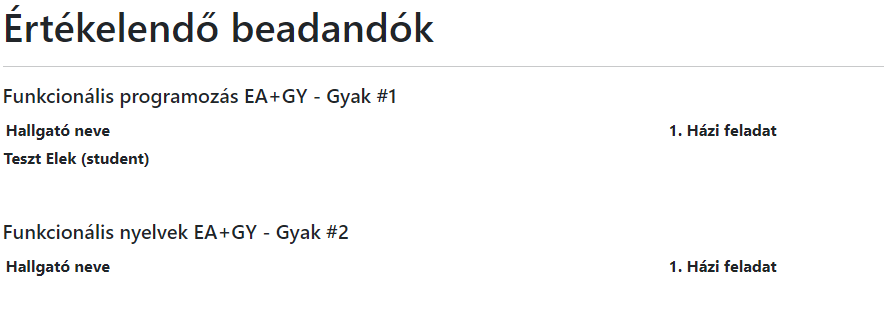
\includegraphics[width=0.75\linewidth]{userguide/instructor-table1}
        \label{subfig:instructor-table1}}
	\hspace{5pt}
	\subfigure[Hallgatói várólista]{
		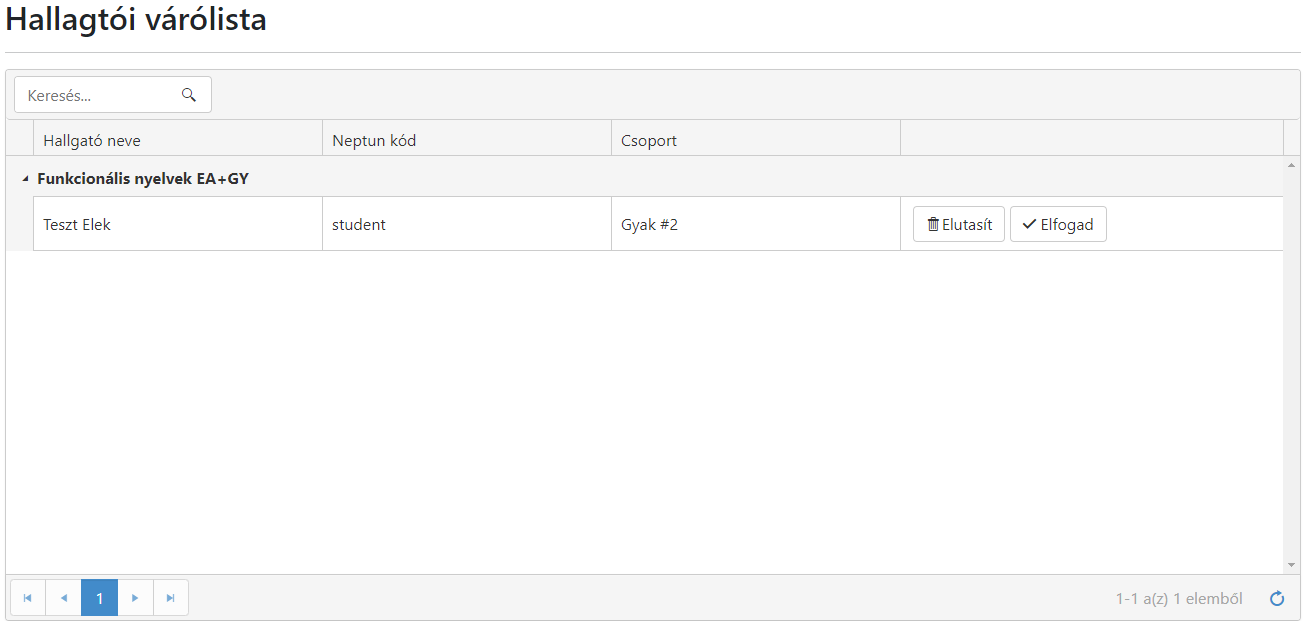
\includegraphics[width=1\linewidth]{userguide/instructor-table2}
        \label{subfig:instructor-table2}}
	\caption{Gyakorlatvezető kezdőoldala}
	\label{fig:instructor-home}
\end{figure}
A gyakorlatvezető az alábbi funkciókat éri el:
\begin{compactitem}
    \item \hyperref[step:instructor-create-assignment]{Feladat kiírása}
	\item \hyperref[step:instructor-pending]{Jelentkezések bírálata}
	\item \hyperref[step:instructor-eval]{Beadott munka értékelése}
\end{compactitem}
\subsubsection{Feladat kiírása}
\label{step:instructor-create-assignment}
Feladatot kiírni a ``Feladat létrehozása'' menüpont alatt tudunk, ahol egy űrlapot találunk (\ref{fig:instructor-create-assignment}). Ahhoz hogy létrehozzunk egy feladatot, a következő információkat szükséges megadnunk:
\begin{compactitem}
    \item A feladat neve
    \item Kezdés és befejezés dátuma
	\item Feladat leírása
	\item Mely csoporthoz legyen létrehozva\footnote{A lenyíló kiválasztó menüben lehetőségünk van több csoportot is kiválasztani}
\end{compactitem}
\begin{figure}[H]
	\centering
	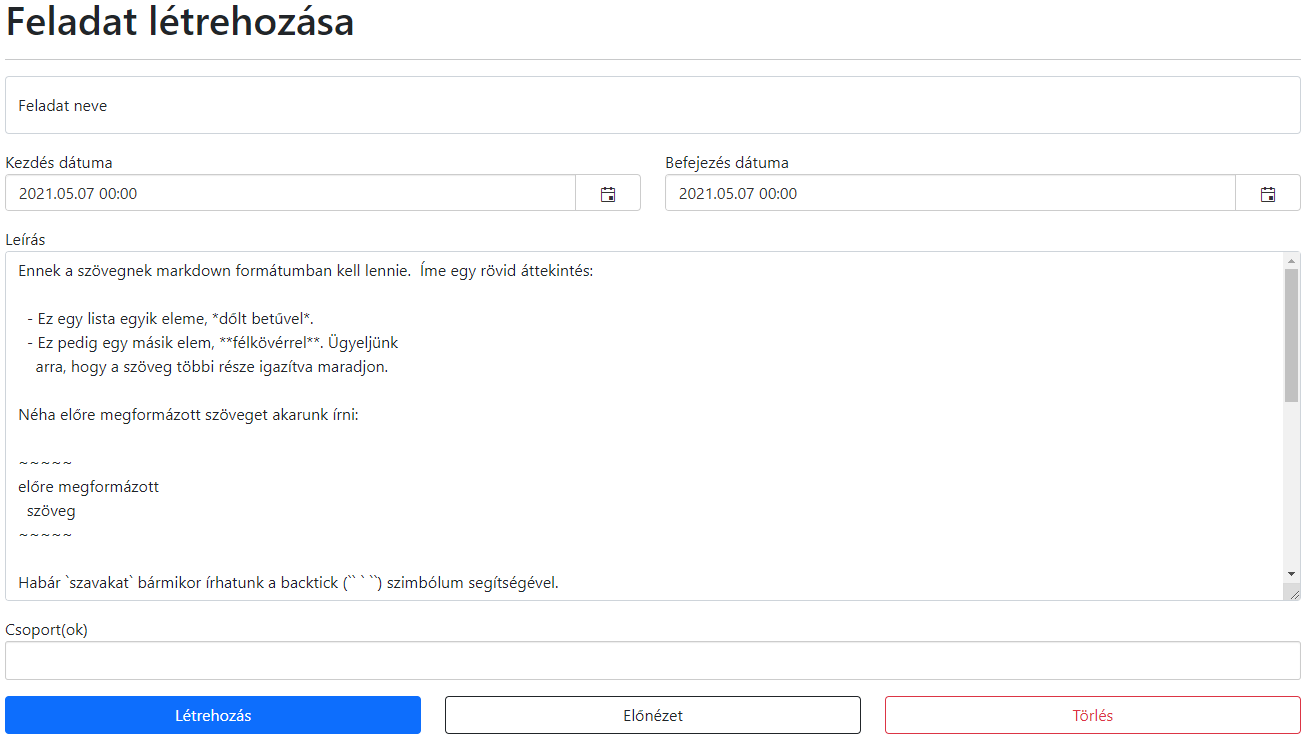
\includegraphics[width=1.0\textwidth]{userguide/instructor-create-assignment}
	\caption{Feladat létrehozás}
	\label{fig:instructor-create-assignment}
\end{figure}
A rendszer támogatja, hogy a feladatnak leírása ne csak egyszerű szöveg legyen. A szövegdobozban megadhatunk \texttt{Markdown} és \LaTeX\ kifejezéseket is. Mielőtt létrehoznánk a feladatot, meg tudjuk tekinteni, hogy a hallgató milyen formában fogja látni a kiírva a feladatot. Így le tudjuk ellenőrizni kényelmesen a feladat leírását, valamint azt is tudjuk ellenőrizni, hogy a \texttt{Markdown} és \LaTeX\ kifejezéseinket helyesen írtuk-e meg. Ha végeztünk, a ``Létrehozás'' gombbal tudjuk elküldeni a rendszernek az adatokat. Az adatokat a rendszer leellenőrzi, az esetleges hibákat jelzi számunkra (\ref{fig:instructor-create-assignment-error}).
\begin{figure}[H]
	\centering
	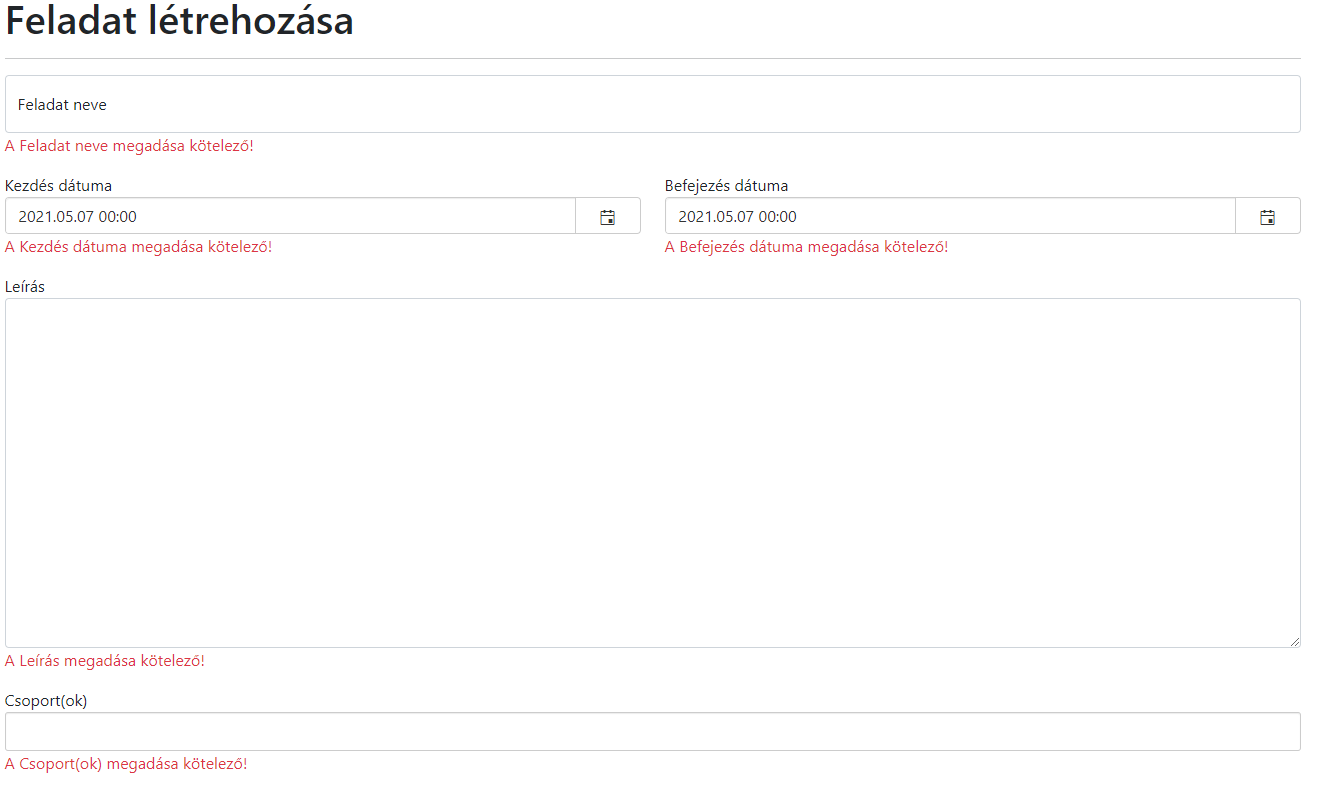
\includegraphics[width=1.0\textwidth]{userguide/instructor-create-assignment-error}
	\caption{Adatok validálása}
	\label{fig:instructor-create-assignment-error}
\end{figure}
\subsubsection{Jelentkezések bírálata}
\label{step:instructor-pending}
Egy hallgatónak a csoportba való jelentkezését a ``Hallgatói várólista'' táblázatában tudjuk megtenni (\ref{subfig:instructor-table2} ábra), az utolsó oszlopban lévő gombok segítségével. Miután elvégeztük a bírálatot, a táblázatból törlődik a jelentkezett hallgató, és az oldal frissítése után, a megfelelő táblázatban látjuk, hogy a hallgatót a rendszer felvette a jelentkezett csoportba.
\subsubsection{Beadott munka értékelése}
\label{step:instructor-eval}
Egy feladatra beadott megoldás értékeléséhez a kívánt feladat oszlopában kattintsunk a \emph{szürke négyzetre}. Ilyenkor a rendszer átirányít minket az értékelő felületre (\ref{fig:instructor-eval-assignment}). A rendszer a felületre a ``Megoldás(ok)'' alatt felsorolja a hallgatónak az összes beadott megoldását a beküldés ideje szerint csökkenően rendezve. Elég egy megoldást értékelnünk, de értékelhetjük az összeset is. Viszont a rendszer a legutolsó értékelést veszi számításba. Ezt fogja a hallgató is látni. A beadott megoldások között a kívánt sorra kattintva tudjuk kiválasztani, hogy melyik megoldást szeretnénk változtatni. Ilyenkor a ``Beadott megoldás'' alatt látjuk, mi a hallgatónak a beadott megoldása. Az értékelésünket az oldal alján található űrlapon tudjuk megtenni. Az értékelés után a rendszer a kezdőoldalra navigál minket. Az értékelt feladatnál a \emph{szürke négyzet} egy \emph{körben lévő pipára} cserélődik.
\begin{figure}[H]
	\centering
	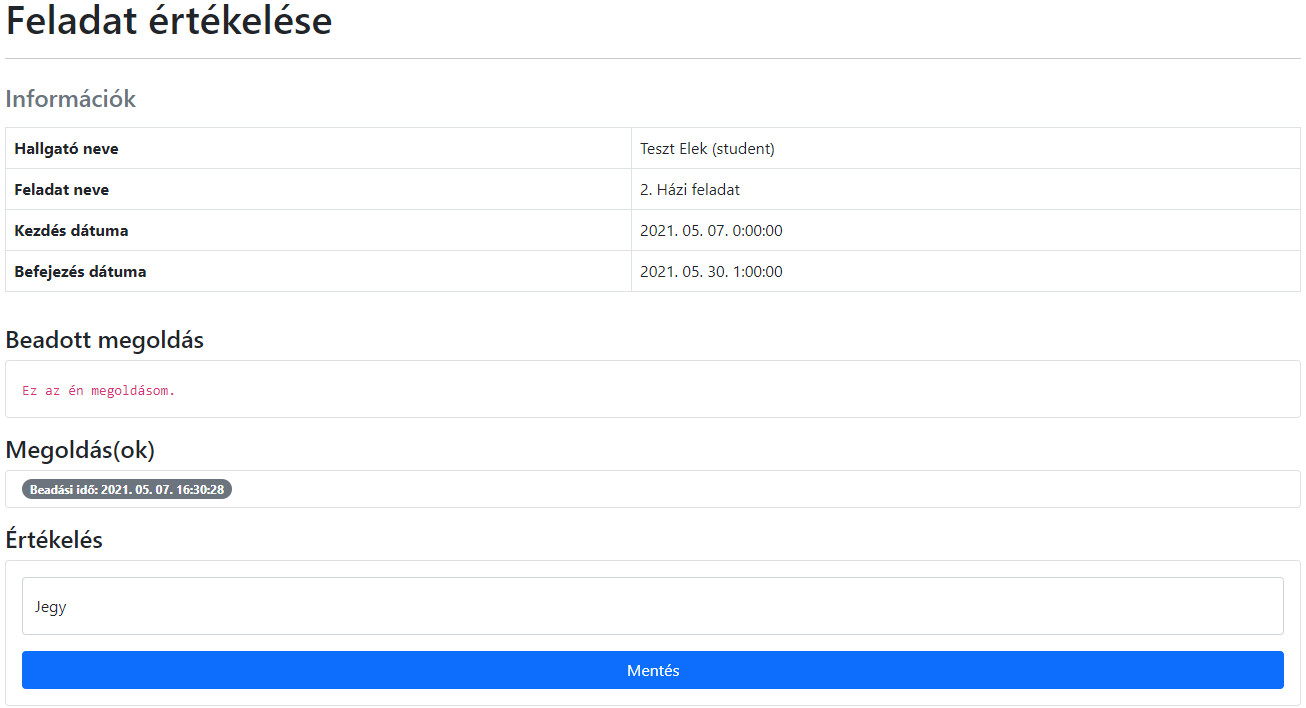
\includegraphics[width=1.0\textwidth]{userguide/instructor-eval-assignment}
	\caption{Feladat értékelése}
	\label{fig:instructor-eval-assignment}
\end{figure}
\subsection{Hallgató}
\label{step:student-role}
Hallgatóként bejelentkezve a \ref{fig:student-home} ábrán látható kezdőoldal fogad minket. A ``Feladatok'' cím alatti táblázatban a hallgató számára listázásra kerül az összes olyan csoportja, ahova elfogadták a jelentkezését. A táblázatban csoportokra lebontva jelennek meg a hallgató számára a kiírt feladatok. A táblázatban egy feladatról a következő információkat láthatjuk: neve, határideje, kapott értékelés.
\begin{figure}[H]
	\centering
	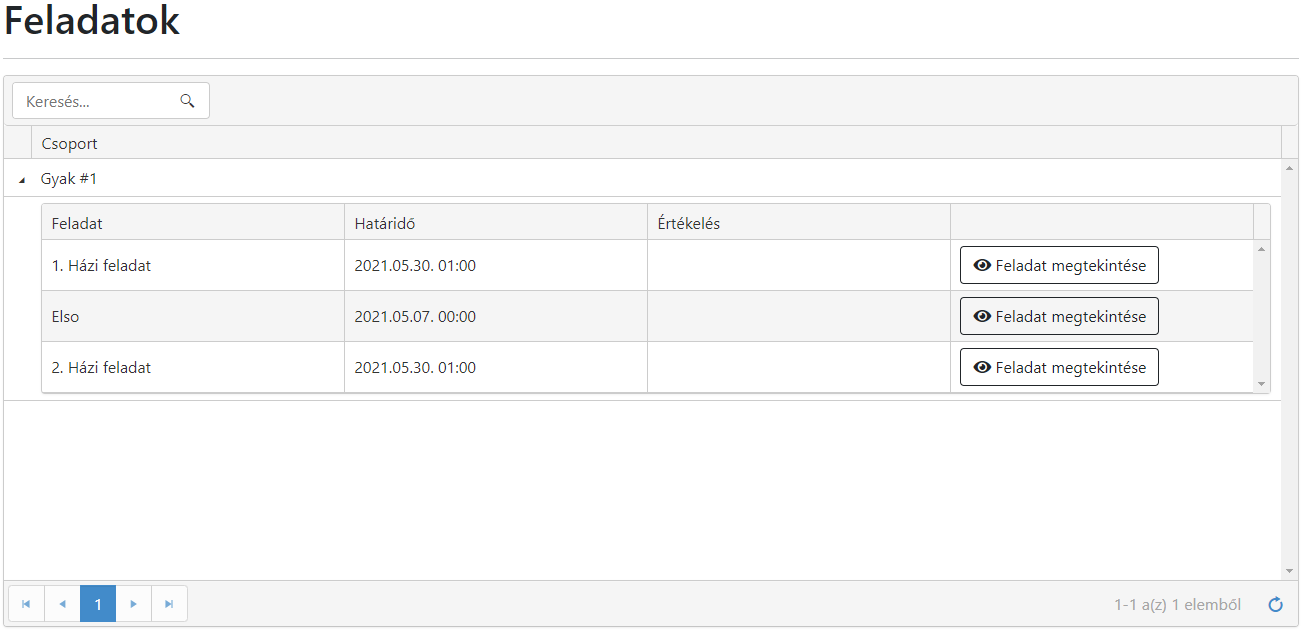
\includegraphics[width=1.0\textwidth]{userguide/student-home}
	\caption{Hallgató kezdőoldala}
	\label{fig:student-home}
\end{figure}
A hallgató az alábbi funkciókat használhatja:
\begin{compactitem}
    \item \hyperref[step:student-course-reg]{Csoportba jelentkezés}
	\item \hyperref[step:student-solution]{Megoldás beadása}
\end{compactitem}
\subsubsection{Csoportba jelentkezés}
\label{step:student-course-reg}
Csoportba jelentkezni a ``Csoport jelentkezés'' menüpontra kattintva tudunk. A rendszer egy űrlapot biztosít számunkra (\ref{fig:student-course-reg} ábra), ahol listázásra kerülnek a rendszerben található csoportok, amelyekre még nem jelentkeztünk. A rendszer lehetőséget biztosít számunkra, hogy akár egyszerre több csoportra is leadjuk a jelentkezésünket. Jelentkezésünket a ``Jelentkezés'' gombbal tudjuk továbbítani a rendszer számára. Az űrlap validálásra kerül, hogy üresen ne tudjuk beküldeni azt. Sikeres jelentkezés esetén a rendszer a kezdőoldalra navigál minket.
\begin{figure}[H]
	\centering
	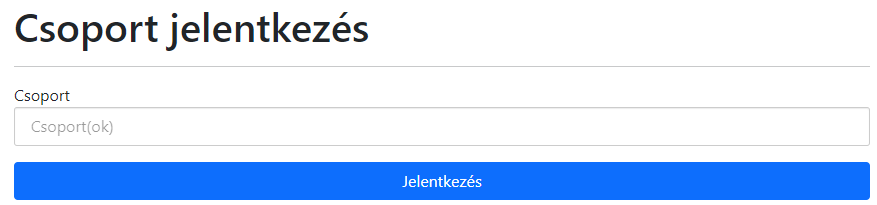
\includegraphics[width=1.0\textwidth]{userguide/student-course-reg}
	\caption{Csoportba jelentkezése}
	\label{fig:student-course-reg}
\end{figure}
\subsubsection{Megoldás beadása}
\label{step:student-solution}
Megoldás beküldéséhez válasszuk ki a kivánt feladatot, amire megoldást szeretnénk beküldeni, majd kattintsunk a ``Feladat megtekintése'' gombra. Ekkor a rendszer egy új ablakban megnyitja a feladatot (\ref{fig:student-submit-sol} ábra). Az oldalon a következő információkat látjuk:
\begin{compactitem}
    \item Határidő visszaszámláló
    \item Feladat neve, leírása
    \item Beküldött megoldások
    \item Űrlap a megoldás beküldéséhez
\end{compactitem}
\begin{figure}[H]
	\centering
	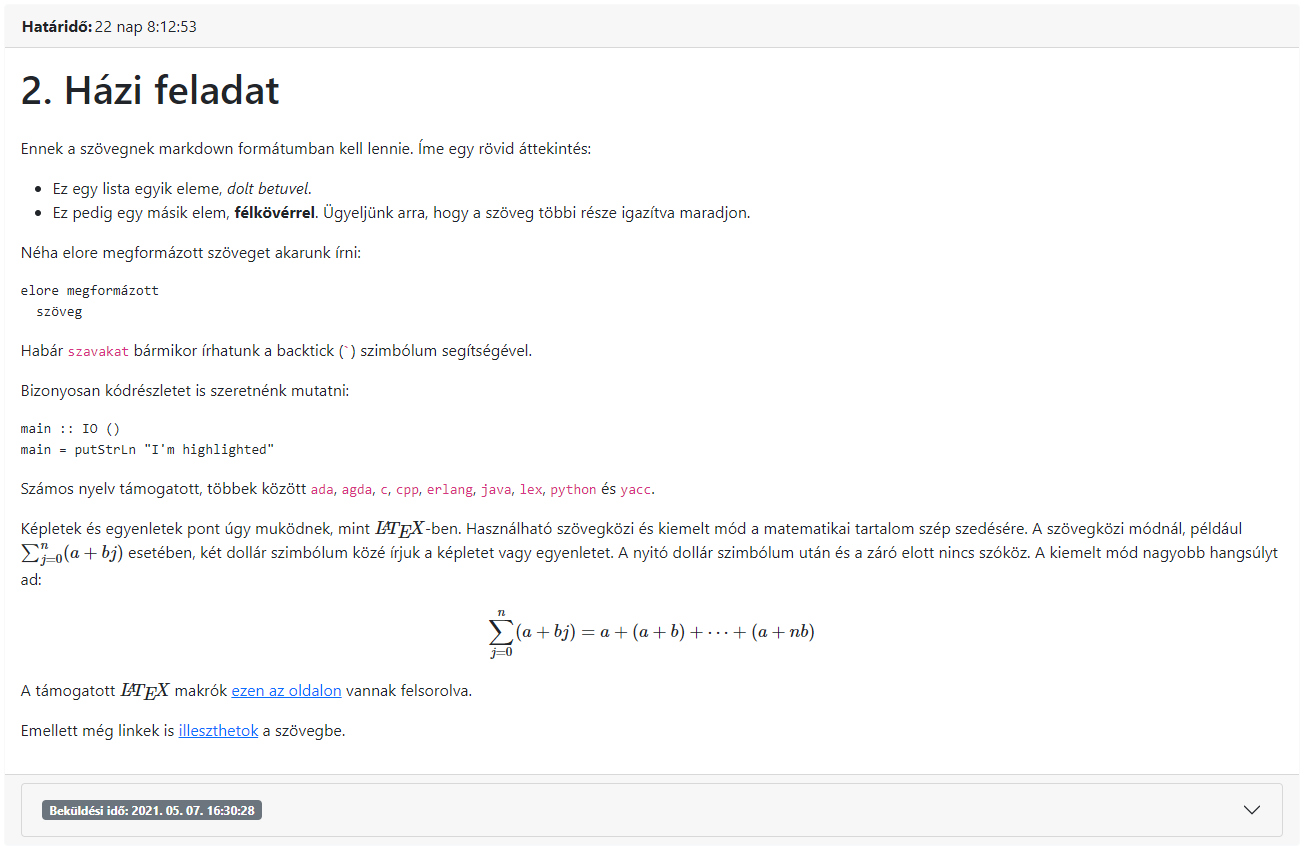
\includegraphics[width=1.0\textwidth]{userguide/student-submit-sol}
	\caption{Feladat megtekintése}
	\label{fig:student-submit-sol}
\end{figure}
\subsection{Mindenki számára elérhető oldalak}
\label{step:mindenkinek-elerheto-oldal}
A rendszerben jelenleg három olyan oldal található, amelyet minden szerepkörben elérhetünk. Az egyik oldal a felhasználónk adatainak megtekintésére szolgál. Ezt a funkciót a menüsoron a nevünkre kattintva tudjuk elérni. Ezen a felületen (\ref{fig:profile} ábra) a következőket tekinthetjük meg a ``Személyes adatok'' cím alatt: név, neptun kód, e-mail cím és a felhasználónkhoz rendelt szerepkörök. Ezen felületen továbbá be tudjuk állítani, hogy a rendszer milyen lokalizációval működjön (magyar és angol). Ezt a megfelelő gombra kattintva tudjuk változtatni.
\begin{figure}[H]
	\centering
	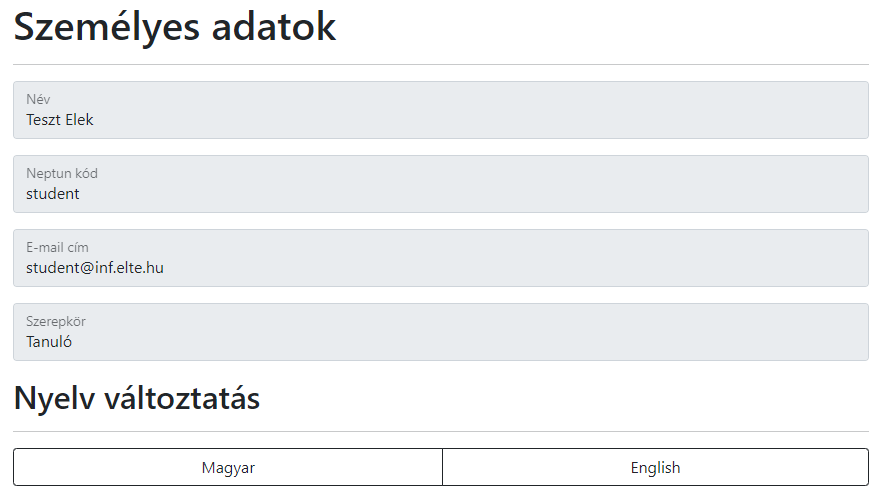
\includegraphics[width=0.8\textwidth]{userguide/profil}
	\caption{Profil oldal}
	\label{fig:profile}
\end{figure}
A másik két oldal az esetleges nem várt hibákról tájékoztat minket. Ezen hibák két kategóriába oszthatók: jogosulatlan kérés a rendszer felé, egyéb nem várt hiba. Jogosulatlan kérés akkor lép fel, ha megpróbálunk a szerepkörünkhöz nem tartozó funkciót elérni a rendszerben. Például: csak hallgatói szerepkörrel rendelkező felhasználóval vagyunk bejelentkezve a rendszerbe és a webcím végén a ``Student''-et lecseréljük ``Admin''-ra. Ezzel olyan kérést indítunk a rendszernek, hogy navigáljon minket a rendszergazdai szerepkörhöz tartozó kezdőoldalra, amihez nincs jogosultságunk, ezért a rendszer megtadja a hozzáférést a kért oldalhoz. Ilyenkor a rendszer az alábbi \ref{fig:access-denied} ábrán látható oldalra navigál minket, ahonnan lehetőségünk van visszatérni a szerepkörünkhöz tartozó kezdőoldalra.
\begin{figure}[H]
	\centering
	
\includegraphics[width=1.0\textwidth]{userguide/access-denied}
	\caption{Jogosulatlan kérés}
	\label{fig:access-denied}
\end{figure}
Egyéb nem várt hiba lehet például, hogy a rendszer nem tud csatlakozni a hozzá tartozó adatbázishoz. Ilyenkor az alábbi \ref{fig:errors} ábrán látható oldalra navigál minket.
\begin{figure}[H]
	\centering
	
\includegraphics[width=1.0\textwidth]{userguide/errors}
	\caption{Egyéb nem várt hiba}
	\label{fig:errors}
\end{figure}